\chapter{Обзор и анализ робототехнических систем, условия их применения}\label{ch:ch1}
Так как целью работы является разработка и исследование робототехнической системы, то первым шагом является рассмотрение других систем, которые используются в предполагаемых местах использования. Критичным является понимание причин использования конкретных движителей в системах, их плюсов и минусов. Необходимо классифицировать существующие типы движителей, понять куда встраивается текущий концепт. Сравнить его с остальными роботами из его семейства. Все это поможет избежать типичные проблемы, связанные с конкретным типом движителя, которые неочевидны по началу разработки.

\section{Классификация машин, использующих ноги в качестве движителя}
Эта классификация основана на работе \cite{Maloletov2015dinamica}. Первые попытки создания многоногих роботов были предприняты в эпоху до нашей эры. В настоящее время можно найти десятки конструкций шагающих роботов, но, как правило, это только экспериментальные прототипы. Из-за обилия различных конструкций, их классификация является нетривиальной задачей. Более того, термин <<ходьба>> имеет различные трактовки, что также является усложняющим фактором для классификации \cite{Bel1984,Brisk2009,Ohom1984,Pavl2013}. 

Определяющей особенностью аппарата, которая в целом позволяет говорить о шагании, является наличие специальных механизмов (ног, шагающих механизмов), которые обеспечивают движение аппарата в результате дискретного взаимодействия с опорой. Под дискретным взаимодействием понимают ситуацию, когда есть моменты времени, в которые механизм контактирует с опорной площадкой, и моменты времени, в которые с опорой механизм не взаимодействует.

Существует несколько видов локомоции. Один из них - ходьба. Этот тип передвижения, когда единовременно земли касается только одна нога. Если возникает ситуация, когда ни одна нога не касается земли, это можно назвать прыжком или бегом \cite{Ohom1984}. Если фаза движения машины с опорой на ноги чередуется с фазой покоя, в которой машина неподвижно лежит на опорной поверхности, то такое движение называется ползанием. Ходьба, прыжки, трусца, бег и ползание предполагают, что соединение ног с опорной поверхностью является не постоянным. Однако ноги могут быть оснащены специальными устройствами - захватами, присосками и т.п., позволяющими устройству осуществлять удерживающие связи с опорной поверхностью. Тип движения такого устройства называется лазанием.

Подводя итог, можно сказать, что классификация следующая. Важно отметить, что в одном экземпляре может сочетаться несколько типов движителей.

Псевдошагающие машины похожи на роботов с ногами, но их ноги всегда обладают опорной поверхностью. Другими словами, эти машины могут только имитировать движение. Одним из распространенных примеров является игрушка, называемая шагающий слон \pic{fig:mechEleph}.


\begin{figure}[H]
\centering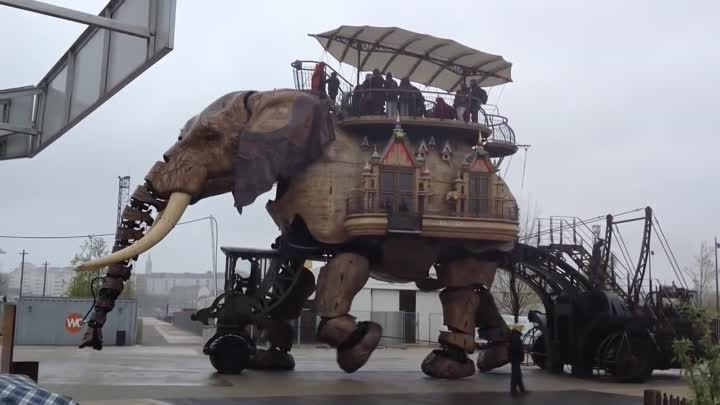
\includegraphics[width=0.8\textwidth]{from_master/mechEleph}
\caption{Механический слон}
\label{fig:mechEleph}
\end{figure}

К классу шагающих машин с дополнительными опорами относятся устройства, имеющие помимо дискретно взаимодействующих с опорной поверхностью шагающих движителей дополнительные механизмы, постоянно контактирующие с опорой. Необходимость в дополнительных опорах обычно возникает тогда, когда шагающих движителей недостаточно для обеспечения устойчивости машины. Чаще всего для этой цели шагающее транспортное средство оснащается колесной тележкой (рис. \ref{fig:Riksha},\ref{fig:steamMan})\cite{briskinSintezCiklovogoShagayushchego2011, Petr1986, Brisk2009,2014,2019,Pavl2013}.

\begin{figure}[H]
\centering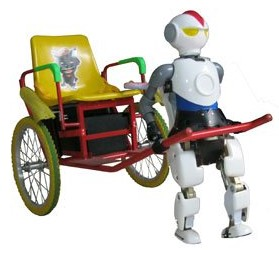
\includegraphics[width=0.6\textwidth]{from_master/Riksha}
\caption{Робот рикша}
\label{fig:Riksha}
\end{figure}

\begin{figure}[H]
\centering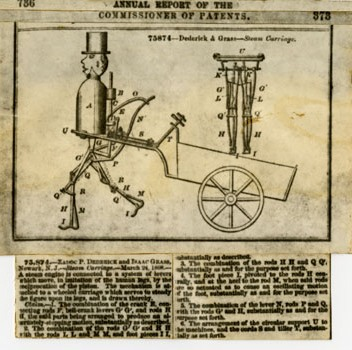
\includegraphics[width=0.6\textwidth]{from_master/steamMan}
\caption{Робот паровой человек}
\label{fig:steamMan}
\end{figure}

Обычно такие машины используются для демонстрации или для отладки системы управления. Использовать их на практике бессмысленно, так как они не имеют никаких преимуществ по сравнению с колесными роботами.

Шагающие машины с циклическими движителями имеет несколько особенностей. Он характеризуется тем, что опорные точки шагающих механизмов движутся по одной и той же траектории относительно корпуса машины, и не решают проблемы адаптации к грунту и выбора точек постановки ног на землю. Такие машины имеют лучшую проходимость по сравнению с колесами меньшее сопротивление движению от земли, лучшее сцепление с основной поверхностью, большие возможности для снижения давления на грунт \cite{cruse2001control}. Примеры машин с циклическими движителями: (рис. \ref{fig:chebishev},\ref{fig:kuban}).

\begin{figure}[H]
\centering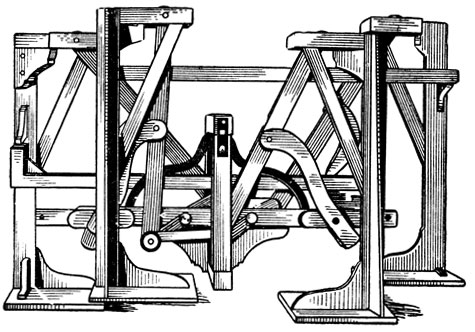
\includegraphics[width=0.6\textwidth]{from_master/chebishev}
\caption{Машина Чебышева}
\label{fig:chebishev}
\end{figure}

\begin{figure}[H]
\centering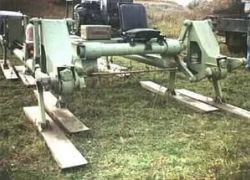
\includegraphics[width=0.6\textwidth]{from_master/kuban.jpg}
\caption{Робот ВолгГТУ Кубань}
\label{fig:kuban}
\end{figure}

Главным преимуществом машин с циклическим шагающим движителем по сравнению с другими шагающими машинами является простота их конструкции и управления.

Ходьба с импровизированным следом --- модификация предыдущего типа движителя и она дает наибольшие преимущества по сравнению с другими заявленными типами движителей. 

Он может принимать постановку ноги на землю, произвольный закон изменения скорости движения ноги как на этапе взаимодействия с землей, так и на этапе переноса. Такие машины значительно превосходят традиционные транспортные средства не только по грунтовой, но и по профильной проходимости. А их главным недостатком является сложность конструкции и системы управления. Это самый многочисленный и разнообразный класс шагающих машин, и большинство приведенных ниже примеров, за исключением специально оговоренных случаев, относятся именно к нему.

Колесно-шагающими машинами традиционно называют класс устройств, в которых колеса шагающих движителей служат упорами. Такие машины могут работать в двух режимах: в режиме колесной машины и в режиме шагающей машины. В первом случае машина движется только с помощью колес. Во втором случае машина совершает шагающие движения, отрывая поочередно колеса от земли и переставляя их на новое место. В этом случае те, что соприкасаются с землей, могут либо блокироваться, либо поворачиваться в соответствии с движением опорных ног.
Есть несколько примеров (рис. \ref{fig:vniitm},\ref{fig:alduro},\ref{fig:athlete}) \cite{germann2001joystick}.

\begin{figure}[H].
\centering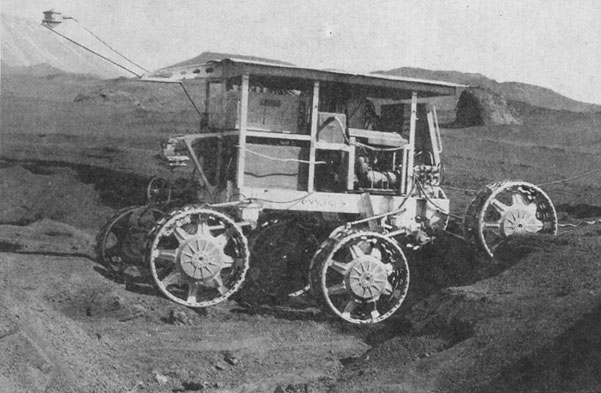
\includegraphics[width=0.6\textwidth]{from_master/vniitm}
\caption{VNIITM}
\label{fig:vniitm}
\end{figure}

\begin{figure}[H]
\centering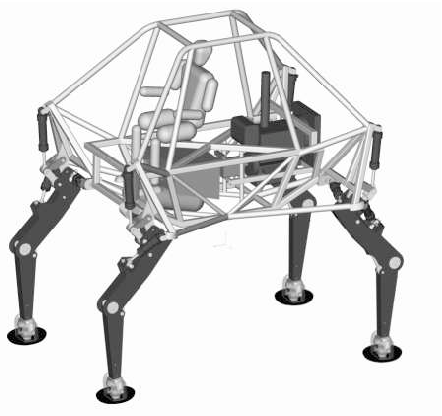
\includegraphics[width=0.6\textwidth]{from_master/alduro}
\caption{Робот Alduro}
\label{fig:alduro}
\end{figure}

\begin{figure}[H]
\centering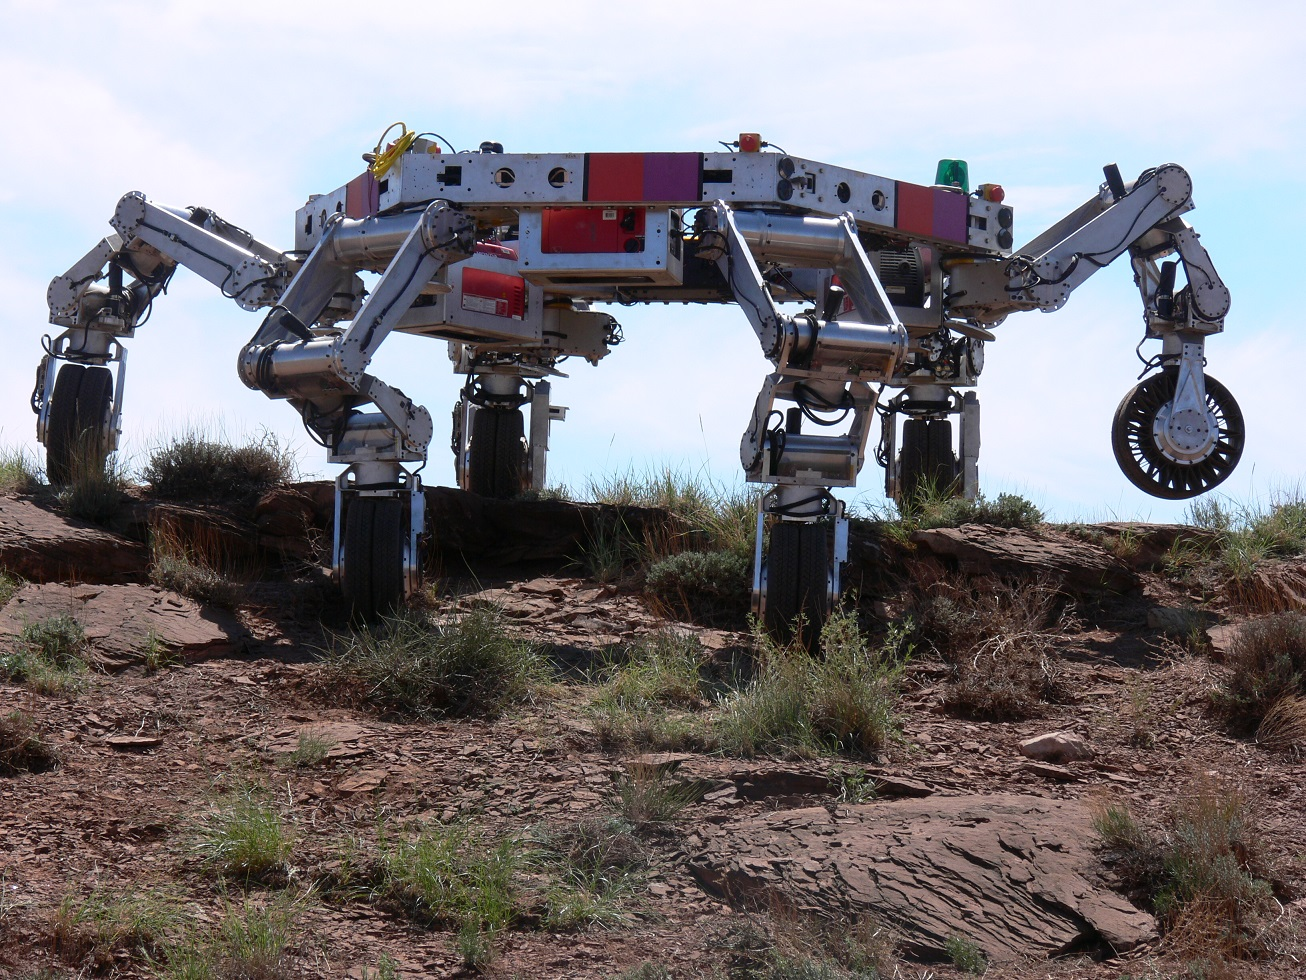
\includegraphics[width=0.6\textwidth]{from_master/athlete}
\caption{Робот Athlete}
\label{fig:athlete}
\end{figure}

Обычно тип движителей <<Прыжки и бег>> может не только прыгать или бегать, но и шагать. Примеры следующие \cite{Pavl2013,volkovaModelirovanieDvizheniyaMnogozvennogo2013,bidgoly2010learning,yacunVibrorobotDlyaVertikalnogo2010} \pic{fig:bigDog}.

\begin{figure}[H]
    \centering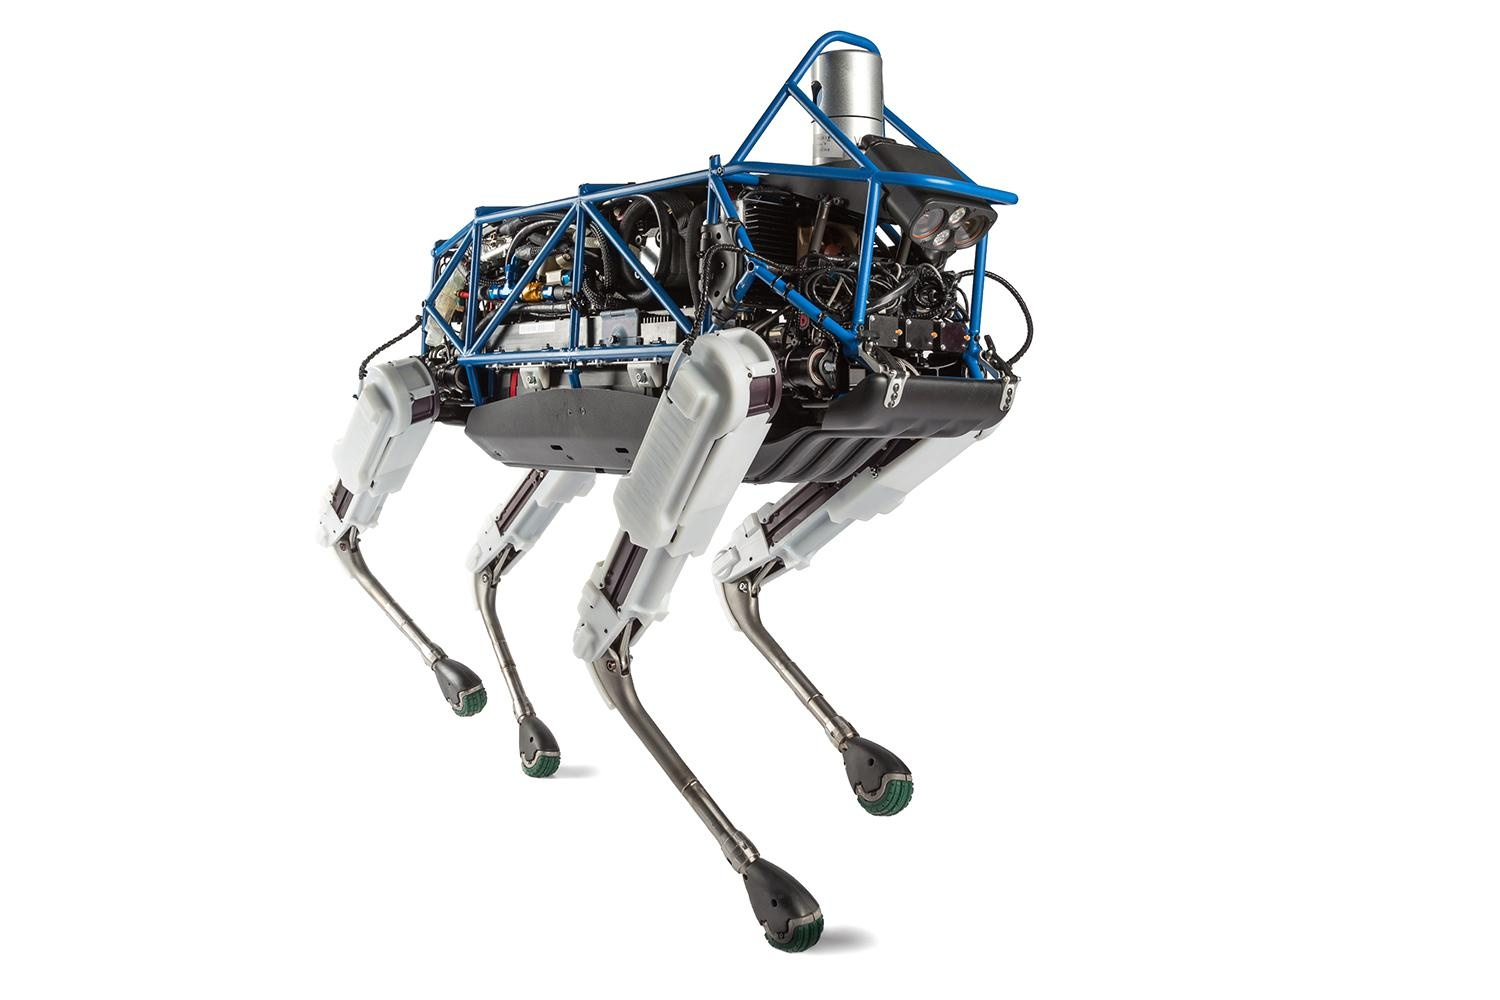
\includegraphics[width=0.8\textwidth]{from_master/bigDog}
\caption{BigDog}
\label{fig:bigDog}
\end{figure}

К машинам ползающего типа в соответствии с приведенным выше определением относится большинство так называемых шагающих экскаваторов \pic{fig:Esh6}. Несмотря на слово "шагающий" в названии, такие машины передвигаются, поднимаясь с помощью ног, и ложатся на опорную поверхность при перестановке ног в новое положение \cite{peters2010prototype,gradeckiySostoyaniePerspektivyRazvitiya2014,bidgoly2010learning}.

\begin{figure}[H]
\centering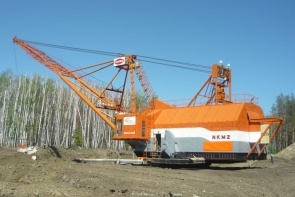
\includegraphics[width=0.7\textwidth]{from_master/Esh6}
\caption{Ползающий экскаватор Российского производства}
\label{fig:Esh6}
\end{figure}

 Специфика взаимодействия с опорной поверхностью и область применения лазающих машин настолько сильно отличаются, что сравнение их показателей (за исключением общетехнических) становится практически бессмысленным. Следует также отметить, что многие ползающие и лазающие роботы не имеют ног или какого-то их подобия, передвигаясь, например, за счет движений гибкого тела.

\begin{figure}[H]
\centering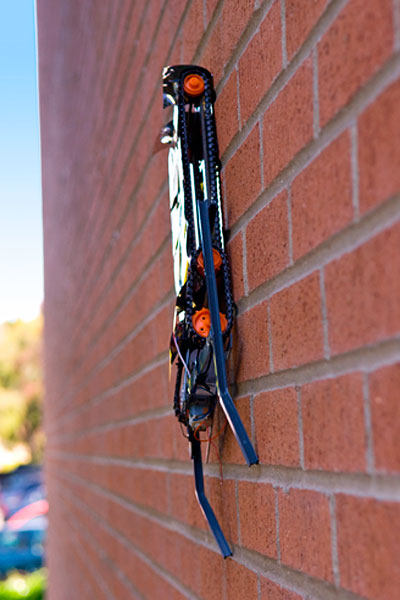
\includegraphics[width=0.45\textwidth]{from_master/brickwall}
\caption{BrickWall робот}
\label{fig:brickwall}
\end{figure}

\begin{figure}[H]
\centering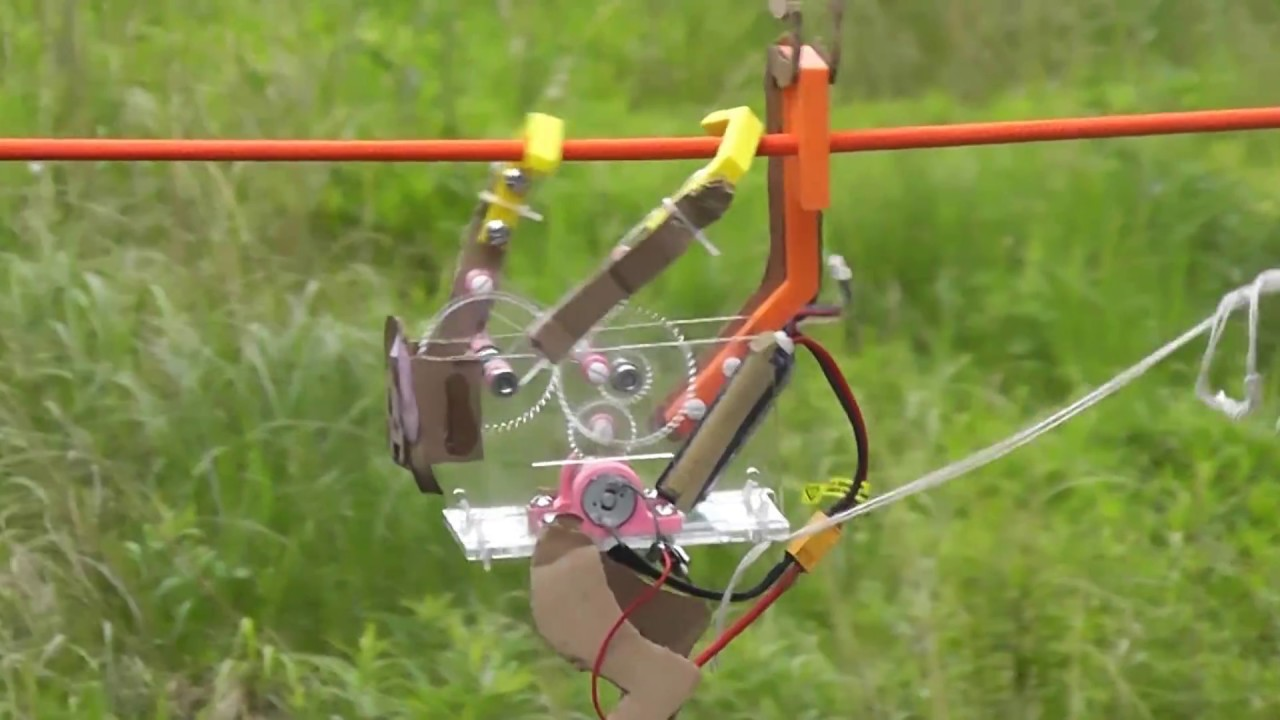
\includegraphics[width=0.7\textwidth]{from_master/ropeClimbing}
\caption{Робот, взбирающийся по канату}
\label{fig:ropeClimbing}
\end{figure}

Согласно этой классификации, робот, который используется в экспериментальной части, относится к категории <<Шагающие машины с циклическим действием движителей>>.

\section{Роботы, которые могут использоваться для исследования пещер}

Исследование пещер естественного происхождения является комплексной задачей, сопряженная со множественными трудностями \cite{Zhang2017a, Frumkin2019}. Деградация сенсоров \cite{Huang2019}, перебои в коммуникации между роботами из-за потери сигналов \cite{Vaquero2018, Thangavelautham2017}, сложный рельеф пещер \cite{Thangavelautham2017}, обилие грязи \cite{Baker2004}, жидких препятствий \cite{Morris2006}, требующие герметизацию корпуса, являются только малой частью встречаемых проблем в пещерах. 

В пещерах возможно встретить почти все типы поверхностей, с которыми приходится сталкиваться роботам в мире. Это и твердые поверхности: мрамор, кварц, базальт. Осадочные горные породы, такие как: мел, гипс, известняк. Часто встречаются водные препятствия — как лужи, так и целы залы, погруженные в воду. Особую опасность для человека вносят сифоны. Скользкие поверхности: лед, мох, глина, а так же разрушаемые поверхности — каменная гряда и паутина \cite{1960,1963,1969,1971}. Знание типов поверхностей и габаритов пещер влияет на типы сенсоров, которые будут установлены на робота и на на необходимую автономность робототехнической системы \cite{Mascarich2018a}. 

Для преодоления сложного рельефа различные роботы, робототехнические системы и типы движителей были предложены исследователями по всему миру \cite{Morris2006a}. Разрушение пещер нежелательно, поэтому роботы, которые для перемещения ломают породу не рассмотрены в данном обзоре \cite{Semini2016}. Для исследования пещер используются, как наземных роботов, так и летающие аппараты, робототехнические комплексы. Из летающего транспорта это коптеры \cite{Papachristos2019,Scaramuzza2014,zinggMAVNavigationIndoor2010} и дирижабли \cite{Huang2019}. Дирижабль намного более автономен и может нести большую нагрузку. Наземных роботов очень много типов, но основными являются: шагающие \cite{Tan2016,Lynch2019} колесные \cite{Molyneaux2016,Vaquero2018}, трековые \cite{Reddy2015} и специфичные. Специфичные движители это движители роботов, которые не поддаются классификации, например змеевидные \cite{Ye2007,Borenstein2007}, шарообразные \cite{Thangavelautham2017,Dubowsky2008,Dang2019} и другие.

Для исследования пещер система роботов является самым эффективным способом разведки. Для использования систем роботов необходимо решать дополнительные задачи, как архитектурного характера, телекоммуникационного и управленческого. Обычно системы состоят из нескольких одинаковых роботов \cite{Vaquero2018}, связка – коптер и шагающий \cite{Chen2010,Cantelli2013}.

Ползающие роботы \cite{Schmidt2013} являются перспективными для исследования пещер по причине их высокой проходимости по узким и невысоким лазам. Ползающие роботы были найдены только для пещер, находящиеся на других планетах \cite{Parness2017}. 

Важным критерием для выполнения задач разведки пещер, является способность перемещаться по вертикальным поверхностям, благодаря высокой адгезии с поверхностью. Это достигается следующими способами: существуют магнитный \cite{Lee2012,tavakoliOmniClimberOmnidirectionalLight2012,Kotay1996,Xu2017}, электрический \cite{Li2017}, негативного давления \cite{Lee2012,tavakoliOmniClimberOmnidirectionalLight2012,Papachristos2019}, пневматический или помощью присосок \cite{Nagakubo1994,Tlale2012}, и с помощью когтей (механическая адгезия) \cite{Parness2017,Bretl2006,SangbaeKim2005,Sintov2011}. Последний способ является самым применимым для пещер, так как стены рельефные.

Навигация в пещерах является нетривиальной задачей, поэтому рассмотрены сенсоры и алгоритмы, а также архитектурные решения используются в представленных выше роботах. Целесообразно рассмотреть работы в близких и смежных областях. К примеру, исследование трубопровода \cite{Savin2017}, завалов после техногенных катастроф. С точки зрения навигации основной проблемой является недостаток света, а также сильной неоднородности территории и обилия гранулированных поверхностей. Решение данной проблем сейчас уделено много внимания, одним из подтверждений данного тезиса является прошедшее соревнование DARPA Subterranean Challenge. В данном направлении используются как лазерные дальномеры (лидары), так и визуальные SLAM алгоритмы \cite{Mascarich2018a,Dang2019a,Fairfield2006,Chhaniyara2012}. С точки зрения архитектуры, наблюдается тенденция к модульности, а также к возможным защитам от потерь робота \cite{Miller2019,weiStudyMineRescue2009}. То есть, если робот был потерян, то остальные роботы все равно должны передавать друг другу данные. Очень важно уметь правильно передвигать робота по сыпучим грунтам, следующие работы посвящены этим проблемам \cite{Tan2016,Savin2017,Chhaniyara2012,Tsounis2019, Li2009,Bjelonic2019,DeViragh2019,Buchanan2019}. Критичным критерием навигации является решение задачи в настоящем времени.

Тип опорной поверхности является одним из ключевых параметров для адоптации управления робота. Зная тип опорной поверхности возможно более оптимально построить маршрут по исследуемой территории. Следующие статьи и их обзоры покрывают основные способы решения данной задачи \cite{wuIntegratedGroundReaction2016,wuTactileSensingTerrainBased2020,luo_robotic_2017}.

Подведя итог, в данном обзоре были представлены причины проблем, возникающие при разведке пещер роботами. Представлены причины, к примеру типы опорных поверхностей, которые влияют на подбор сенсоров и алгоритмов, а также сделаны выводы как это влияет на робототехническую систему. После этого показаны решения, предложенные исследователями по всему миру, связанные с навигацией, подбором движителя, выбором сенсоров и архитектурными решениями, дающие надежную систему. 

\section{Исследования роботов с цикловым движителем}
Одной из разновидностью роботов с цикловым движителем является гесаподы. Гексапод это разновидность мобильных шагающих роботов с 6ью конечностями. Такая форма демонстрирует качественное поведение сороконожки. То есть, чаще всего роботы гексаподы --- биомиметические роботы, то есть роботы, вдохновленные природой.

Не смотря на это, существуют интересные попытки создать гибриды между колесными роботами и многоножками, чтобы получить "лучшее из обоих миров".

Boston Dynamics RHex \cite{Altendorfer2001} - это шестиногий робот \pic{fig:rhex}, тело которого похоже на робота, который используется в экспериментальной части. Независимо управляемые ноги создают специальные походки, которые перемещают его по неровной местности, такой как лестница, каменная гряда и т.д. Данный робот умеет прыгать. Форма ног обеспечивает плавность движений. Однако у робота есть и ряд недостатков. Прежде всего, это высокое энергопотребление, так как он содержит шесть двигателей. Кроме того, у этого робота есть некоторые трудности с управляемостью. 

\begin{figure}[H]
    \centering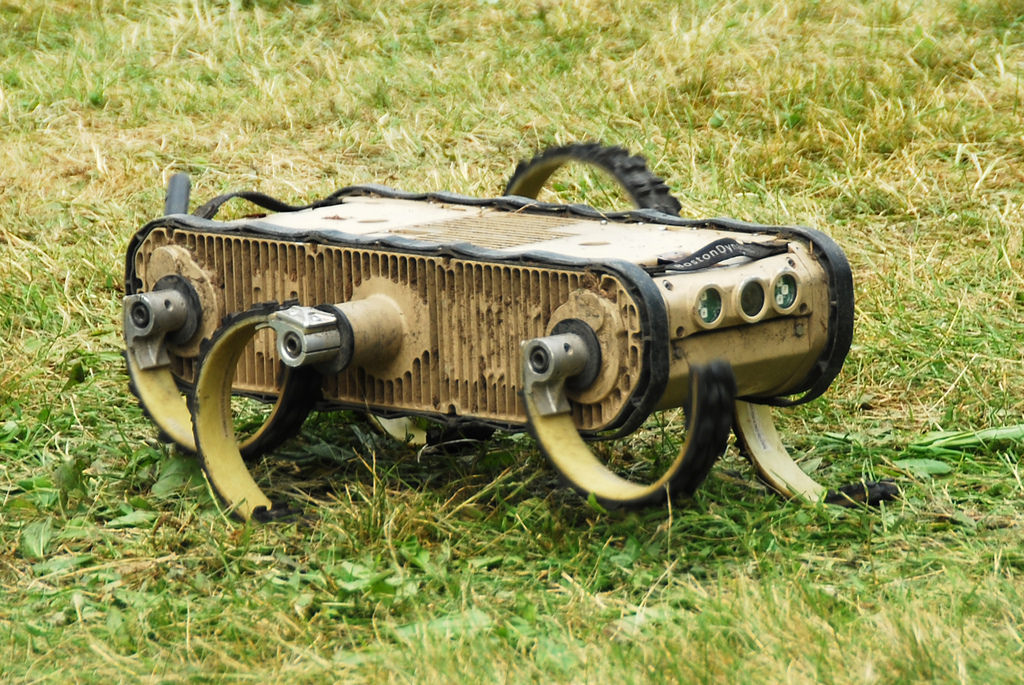
\includegraphics[width=0.4\textwidth]{from_master/rhex}\\
    \caption{Boston Dynamics робот RHex}
    \label{fig:rhex}
    \end{figure}

Gakken Mechamo Centipede \cite{millerExtremeMakeoverHeianera2008, Miller2019} - робот \pic{fig:gakken}, который имеет схожую кинематическую схему с СтриРусом. Большое количество ног может обеспечить ему хорошую проходимость на пересеченной местности, и потеря ноги не будет критичной для робота. Однако это увеличило количество компонентов робота, что удорожает производство и техническое обслуживание. Минусом данной конструкции это малая длина педипулятора снижает возможности передвижения по пересеченной местности.
\begin{figure}[H]
    \centering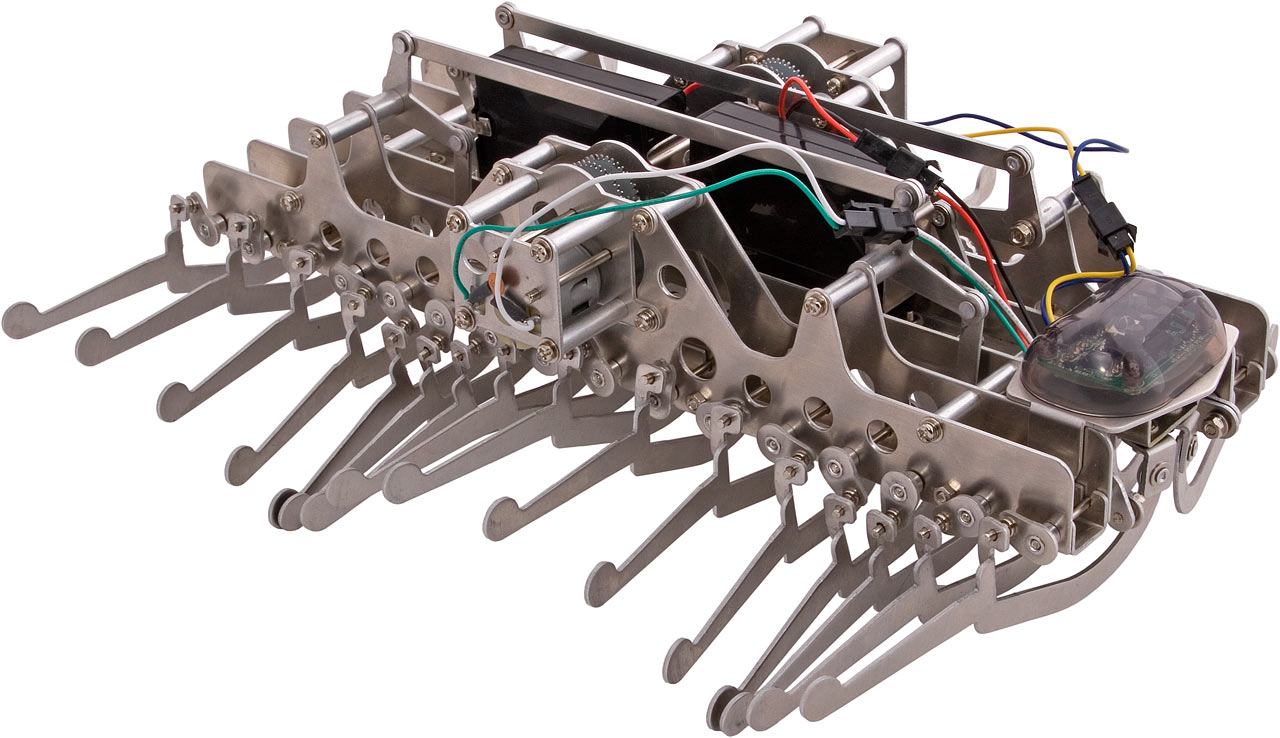
\includegraphics[width=0.5\textwidth]{from_master/gakken}\\
    \caption{Gakken Mechamo Centipede робот}
    \label{fig:gakken}
    \end{figure}

Quattroped и TurboQuad \cite{shenDesignLegwheelHybrid2009, Chen2014, Chen2017} --- это роботы, трансформирующие колеса в ноги \pic{quatro}. Когда он использует ноги, его кинематическая схема похожа на робота RHex, в случае режима работы колес он похож по управлению на радиоуправляемую машинку. Данный инженерный прием обеспечивает высокую скорость на ровной местности, но конструкция робота становится конструкционно сложной, что снижает надежность системы. У робота 4 ноги, что делает его неустойчивым в некоторых ситуациях.

\begin{figure}[H]
    \begin{subfigure}{0.49\textwidth}
    \centering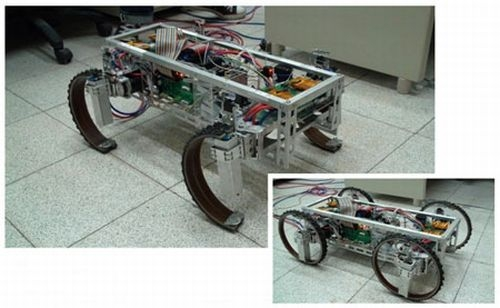
\includegraphics[width=0.9\textwidth]{from_master/quattroped}\\
    \caption{Quattroped robot}
    \label{fig:quattroped}
    \end{subfigure}
    \begin{subfigure}{0.49\textwidth}
    \centering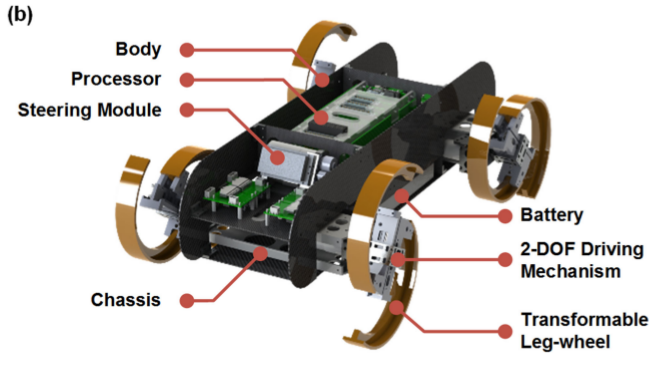
\includegraphics[width=0.9\textwidth]{from_master/turboquad}\\
    \caption{TurboQuad robot}
    \label{fig:turboquad}
    \end{subfigure}
    \caption{Quattroped семья роботов}
    \label{quatro}
    \end{figure}

Whegs \cite{schroerComparingCockroachWhegs2004} \pic{fig:whegs} использует стратегию локомоции, которая сочетает простоту колеса с преимуществами преодоления препятствий ногой. Робот обладает сегментированным телом, что позволяет ему при малой длине педипуляторов соперничать по проходимости с остальными представителями данного класса роботов. Сегментированность делает робота более сложным в производстве и управлении.

\begin{figure}[H]
\centering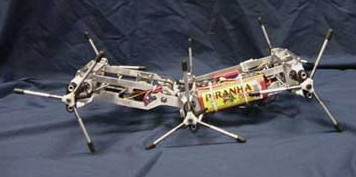
\includegraphics[width=0.7\textwidth]{from_master/whegs2.jpg}\\
\caption{Whegs II}
\label{fig:whegs}
\end{figure}

Сравнительный анализ между представленными выше роботами приведен в таблице \ref{tabular:robot_comparison}.
\begin{table}[H]
    \centering
\caption{Сравнительный анализ гесаподов}
\label{tabular:robot_comparison}
% \small
\begin{tabular}{l|c|c|c|c}
\toprule
\toprule
\rowcolor{Gray}
 Параметры, СИ & RHex & \makecell{Gakken \\ Mechamo\\ Centipede} &  \makecell{Quattroped} & \makecell{Whegs II}\\
 \hline
Длина, мм & 540 & 320 & 600 & 470 \\ 
  \rowcolor{LightGray}
 Ширина, мм & 200 & 140 & 190 & 360 \\
 Высота, мм & 127 & 100 & 140 & 50 \\
  \rowcolor{LightGray}
 Масса, кг & 8.2 & 1.1 & 8.6 & 3.86 \\ 
 Количество ног & 6 & 32 & 4 & 18 \\
  \rowcolor{LightGray}
 Высота ноги, мм & 175 & 50 & 175 & 100  \\
 Масса ноги, кг & 0.1 & 0.02 & 0.38 & 0.05 \\
  \rowcolor{LightGray}
 Скорость, м/с & 1.6 & 0.1 & 2 & 1.5 \\
\bottomrule
\bottomrule
\end{tabular}
% \end{center}
\end{table}

Все эти роботы, кроме Gakken Centipede, были созданы для разведки, в том числе и пространствах искусственного происхождения, и значения параметров можно легко объяснить. Ширина должна быть меньше ширины дверного проема. Еще лучше, если ширина робота будет меньше 2/3 размера двери, и все прототипы удовлетворяют этому условию. При навигации внутри помещений длина также должна быть минимально возможной, иначе он не сможет передвигаться в коридорах и тесных помещениях. Масса зависит от других параметров. Высокая скорость не нужна в помещениях и опасных зонах. 

Похожие роботы, такие как Boston Dynamics RHex \cite{Altendorfer2001}, Gakken Mechamo Centipede \cite{Miller2019}, Quattroped and TurboQuad \cite{Chen2011,Chen2014,Chen2017}, а так же Whegs \cite{schroerComparingCockroachWhegs2004} были рассмотрены. Рассмотрев других представителей выбранного класса роботов и определив причины таких параметров, было решено, что робот должен быть в длину меньше метра, в ширину --- меньше 70 см (стандартная ширина дверного проема). Иметь меньше 32 лапок и высота лапки должна быть больше 10 см.


\section{Описание пещеры}
Пещера -- полость в верхней части земной коры, сообщающаяся с поверхностью одним или несколькими входными отверстиями. Пещеры естественного происхождения бывают: карстовые, тектонические, эрозионные, ледниковые и вулканические. В них могут быть найдены следующие структуры поверхностей:
\begin{itemize}
    \item твердые породы, прочные -- мрамор, кварц, базальт (магма) \pic{fig:solid_surfaces};
    \item твердые породы, мягкие -- мел, гипс, соль, известняк \pic{fig:solid_surfaces};
    \item сыпучие грунты -- песок, глина, снег \pic{fig:running_soils};
    \item водные преграды -- как и лужи (малый слой воды), залы, погруженные под воду, сифоны \pic{fig:water_obstacles};
    \item скользкие поверхности -- отложения мха и плесени, лед \pic{fig:slippery_surfaces};
    \item разрушаемые поверхности -- каменная гряда, паутина.
\end{itemize}


\begin{figure}[H]
\begin{subfigure}{0.49\textwidth}
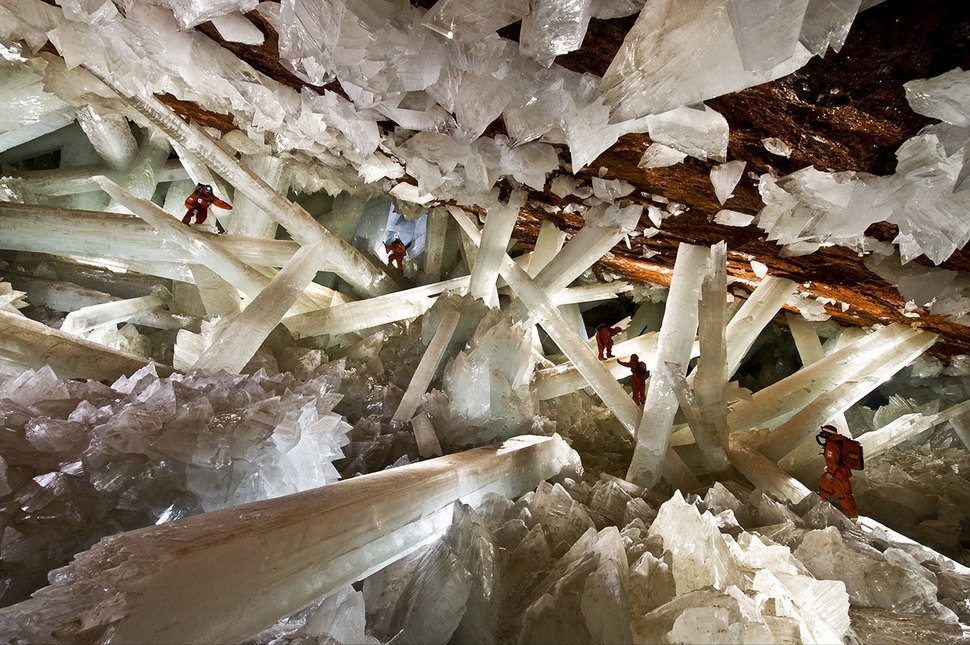
\includegraphics[width=0.99\textwidth]{surface_types/crystal.png}\\
\caption{Кристаллы}
\label{fig:crystal}
\end{subfigure}
\begin{subfigure}{0.49\textwidth}
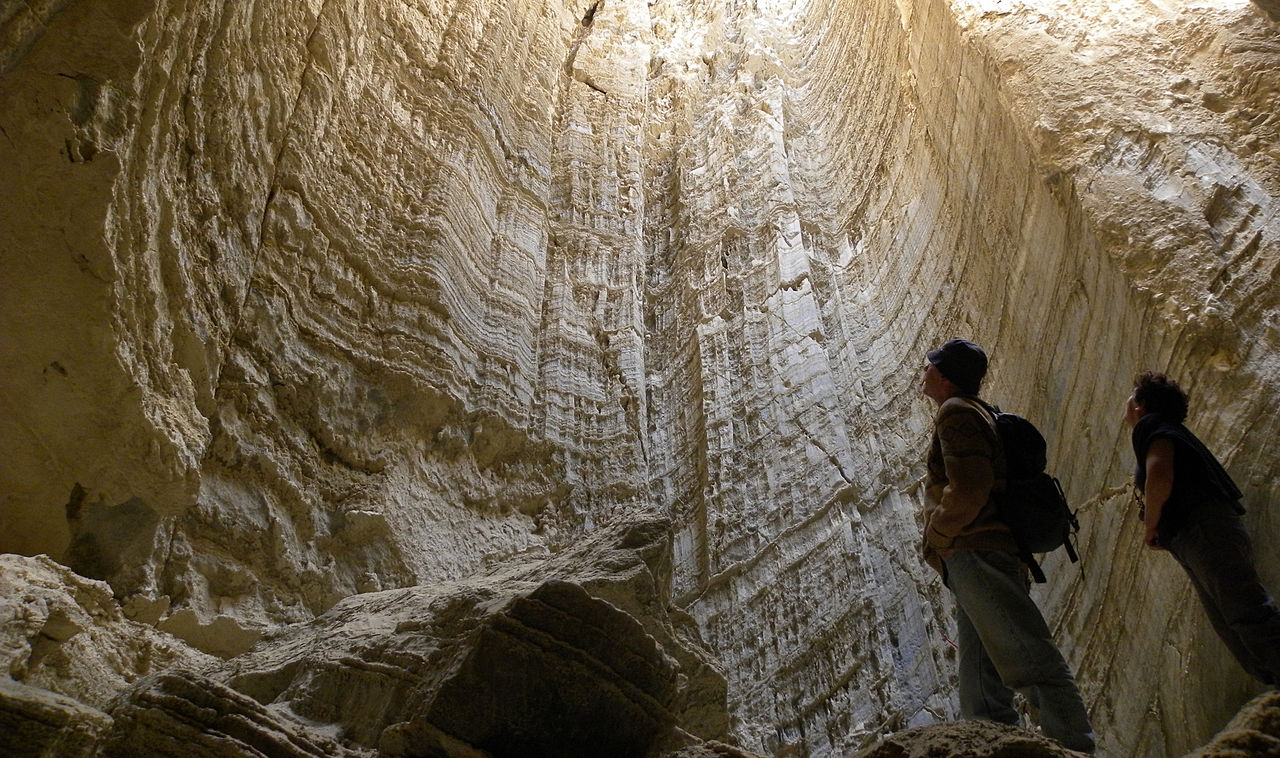
\includegraphics[width=0.99\textwidth]{surface_types/salt.jpg}\\
\caption{Солевые отложения}
\label{fig:salt}
\end{subfigure}

\begin{subfigure}{0.49\textwidth}
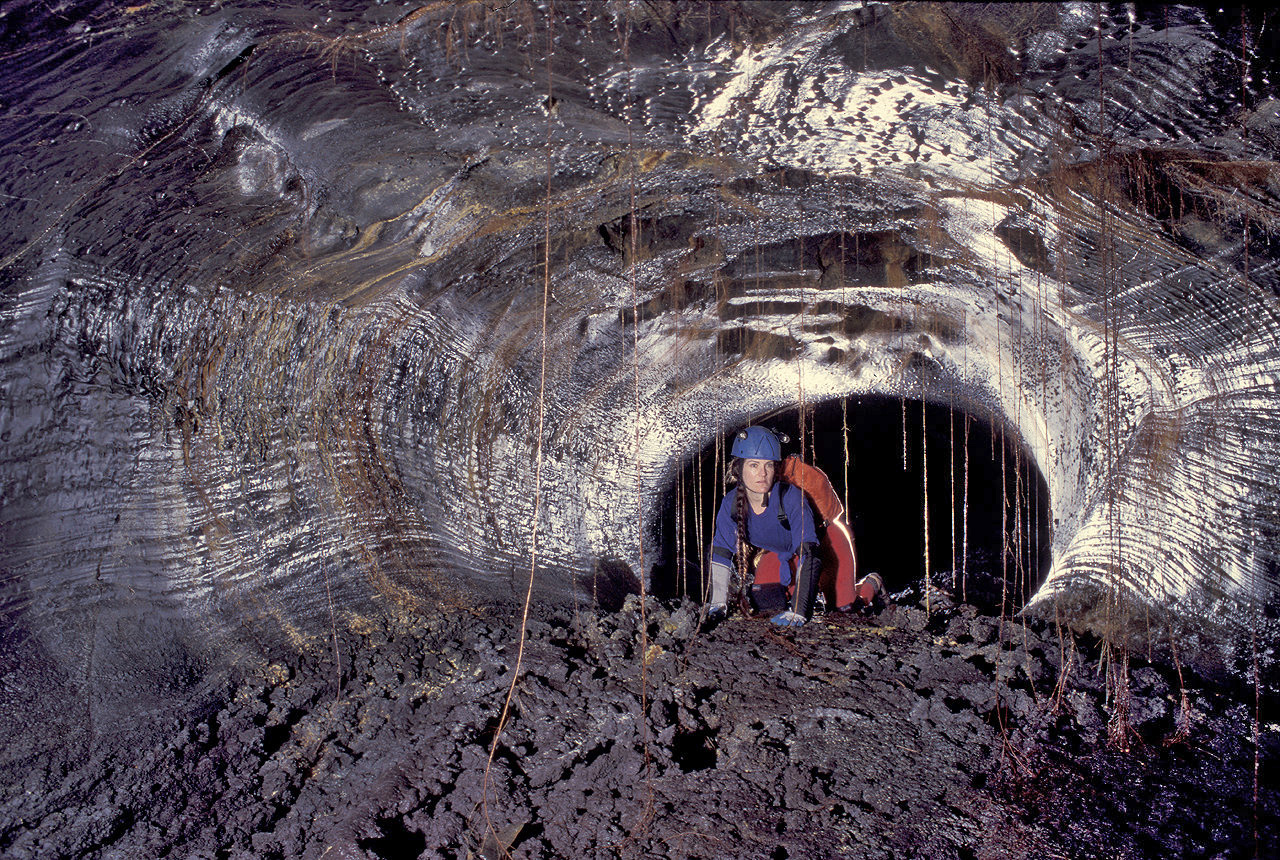
\includegraphics[width=0.99\textwidth]{surface_types/lava.jpg}\\
\caption{Магма}
\label{fig:lava}
\end{subfigure}
\begin{subfigure}{0.49\textwidth}
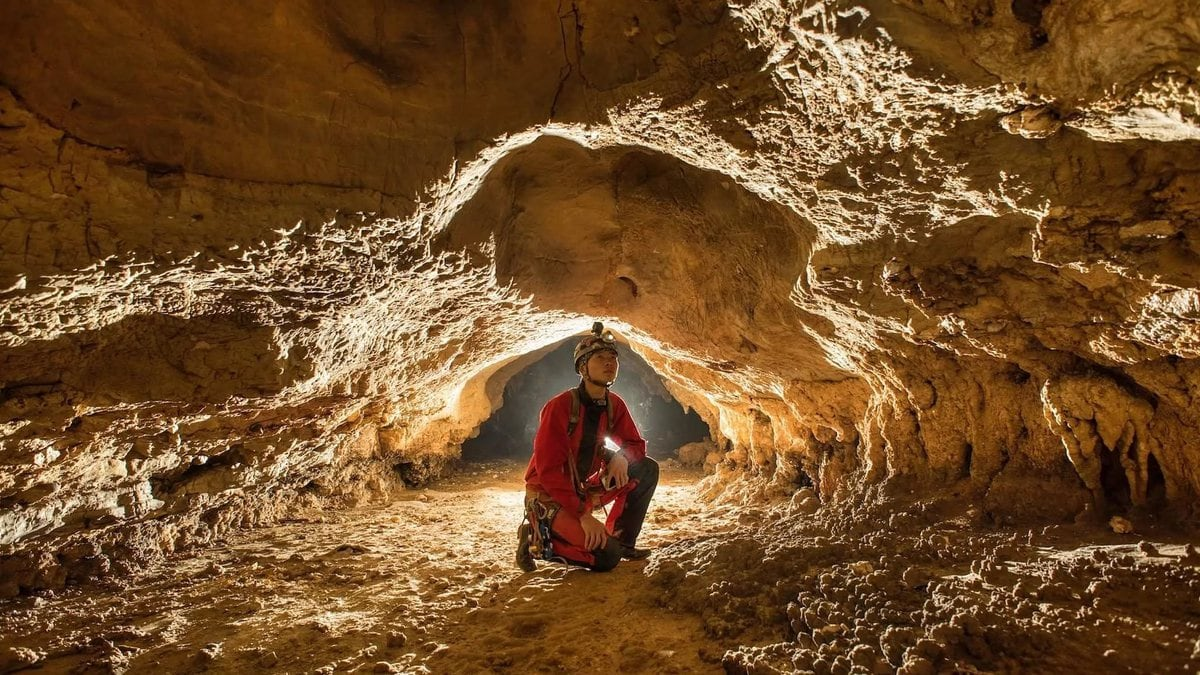
\includegraphics[width=0.99\textwidth]{surface_types/limestone.png}\\
\caption{Известняк}
\label{fig:limestone}
\end{subfigure}
\caption{Твердые поверхности}
\label{fig:solid_surfaces}
\end{figure}

\begin{figure}[H]
\begin{subfigure}{0.49\textwidth}
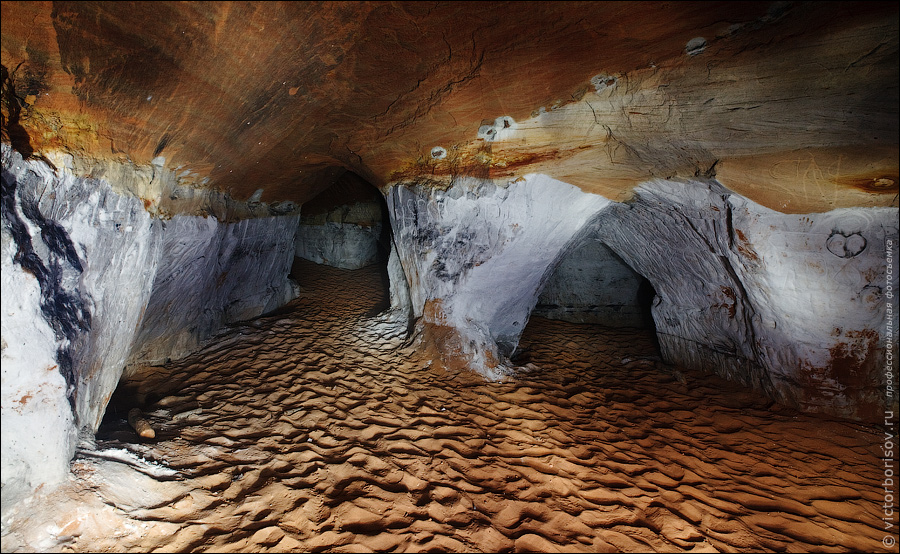
\includegraphics[width=0.99\textwidth]{surface_types/sand.jpg}\\
\caption{Песок}
\label{fig:sand}
\end{subfigure}
\begin{subfigure}{0.49\textwidth}
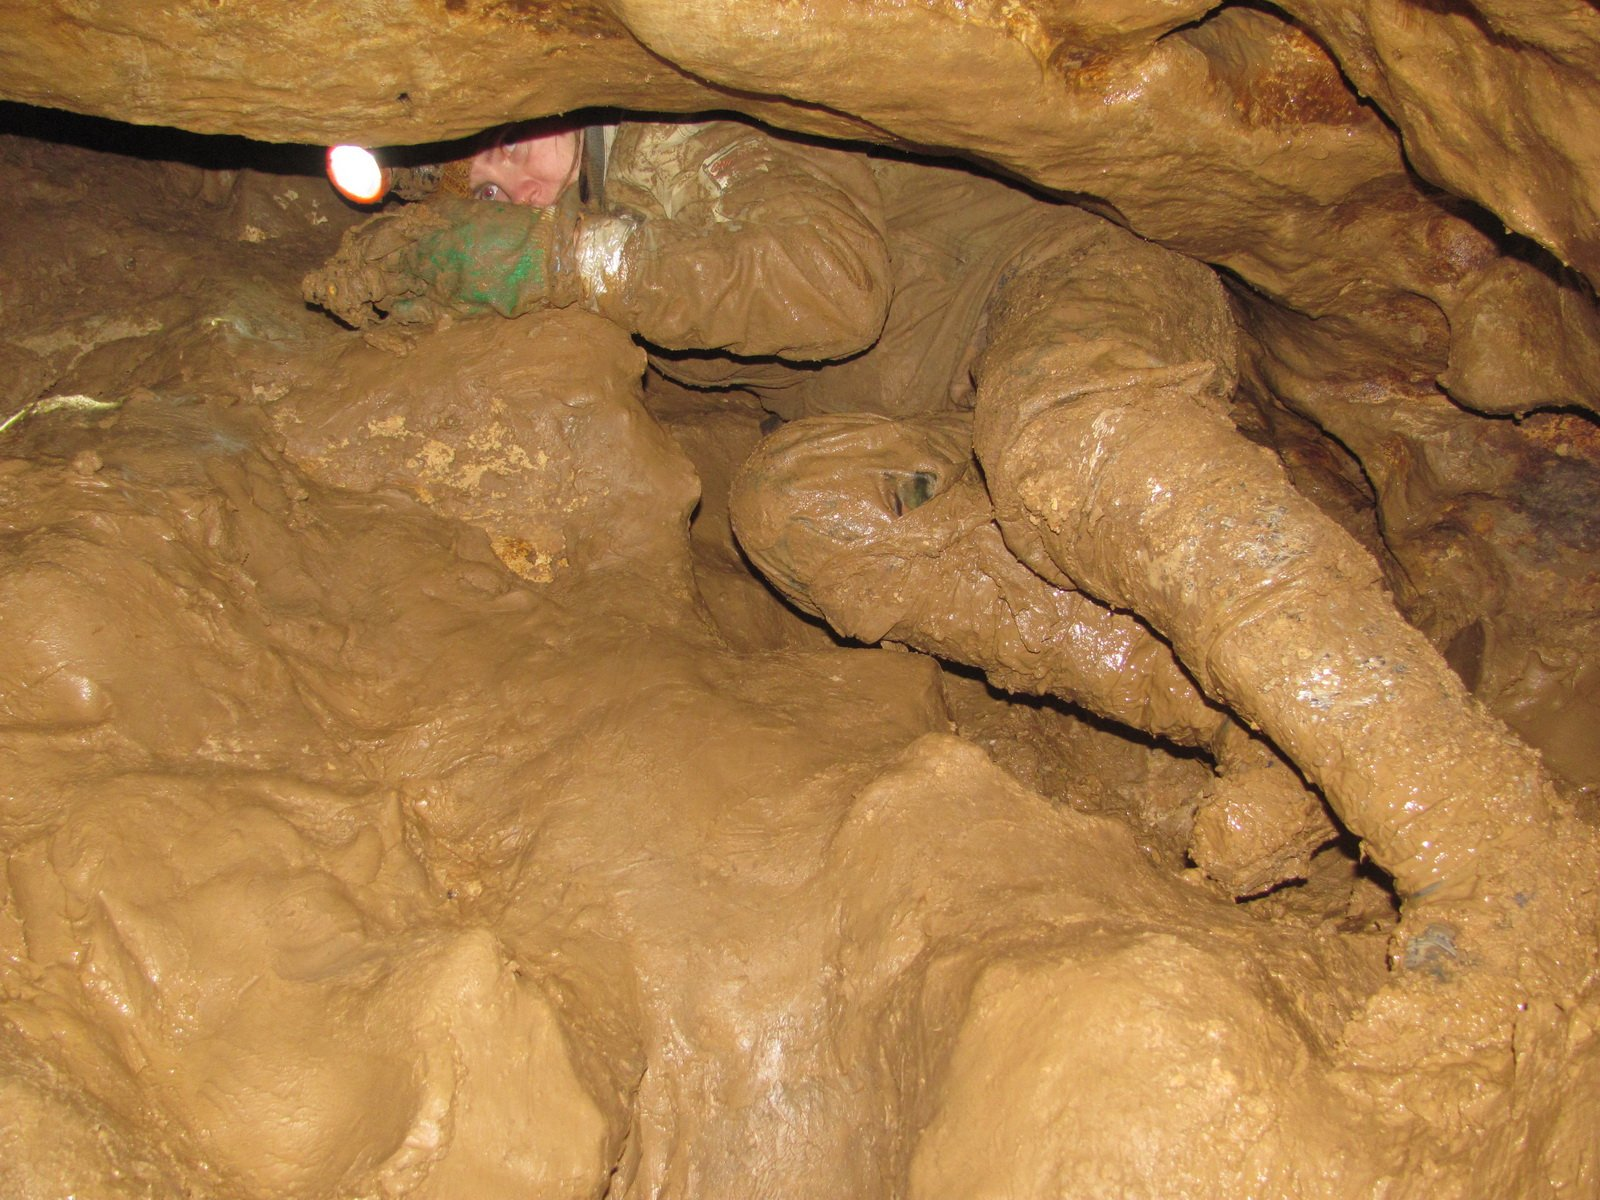
\includegraphics[width=0.89\textwidth]{surface_types/clay.jpg}\\
\caption{Глина}
\label{fig:clay}
\end{subfigure}
\caption{Сыпучие грунты}
\label{fig:running_soils}
\end{figure}

\begin{figure}[H]
\begin{subfigure}{0.49\textwidth}
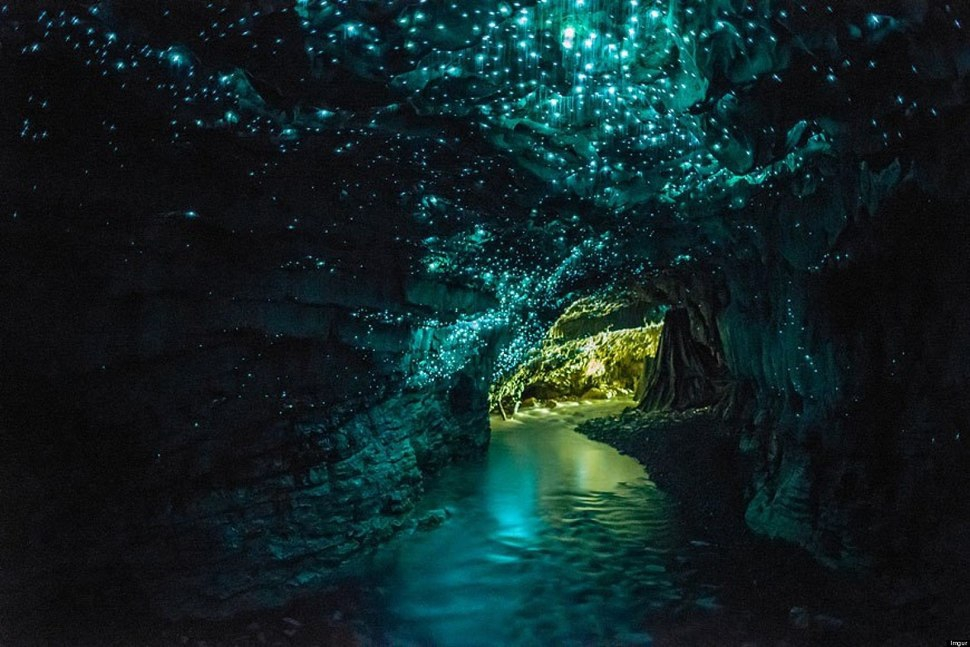
\includegraphics[width=0.99\textwidth]{surface_types/splash.png}\\
\caption{Лужа}
\label{fig:splash}
\end{subfigure}
\begin{subfigure}{0.49\textwidth}
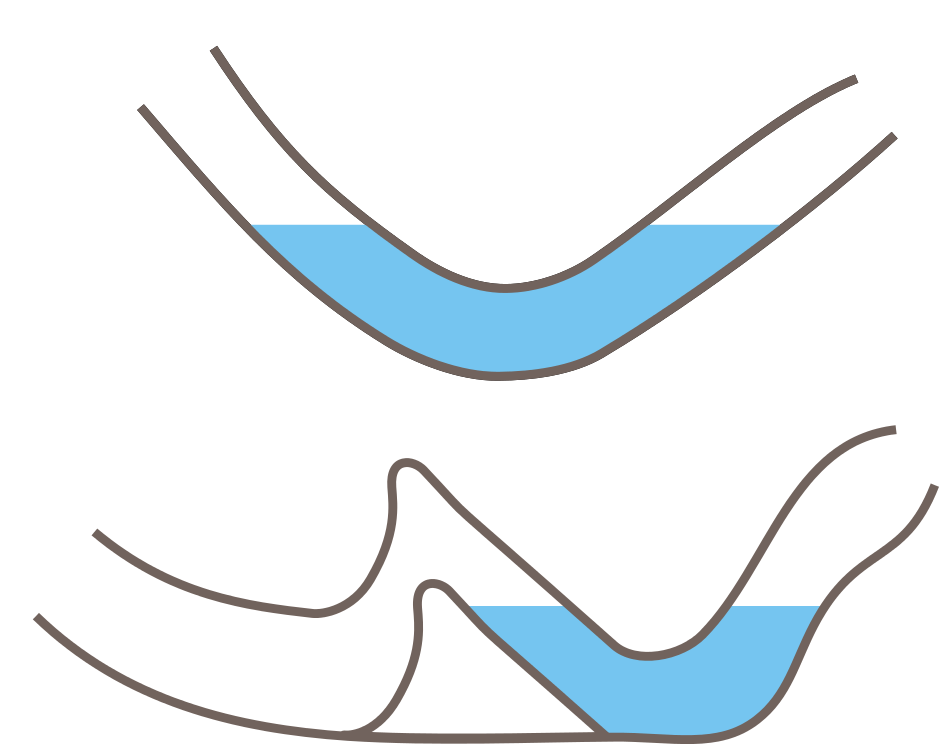
\includegraphics[width=0.84\textwidth]{surface_types/siphon.png}\\
\caption{Сифон}
\label{fig:siphon}
\end{subfigure}
\caption{Водяные препятствия}
\label{fig:water_obstacles}
\end{figure}

\begin{figure}[H]
\begin{subfigure}{0.49\textwidth}
\centering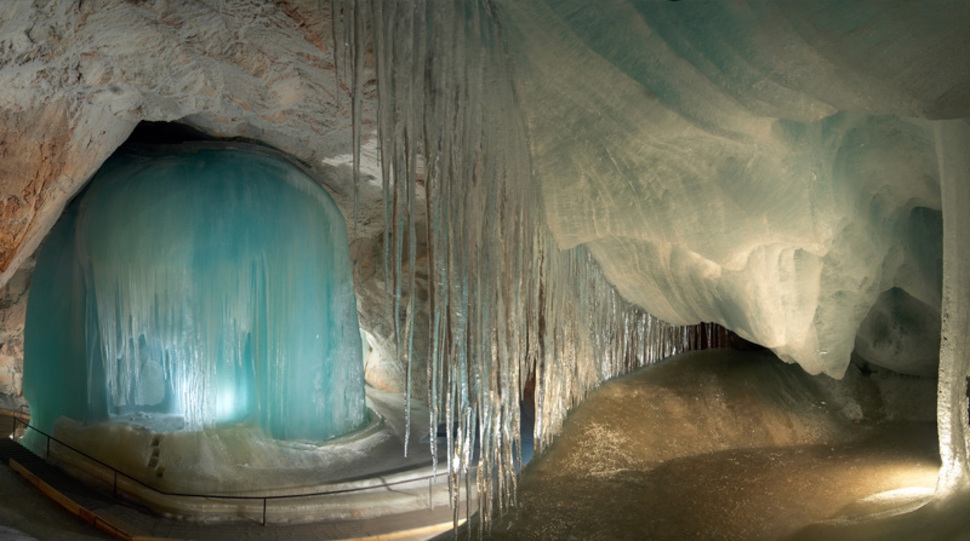
\includegraphics[width=0.99\textwidth]{surface_types/ice.png}\\
\caption{Ледяная пещера}
\label{fig:icee}
\end{subfigure}
\begin{subfigure}{0.49\textwidth}
\centering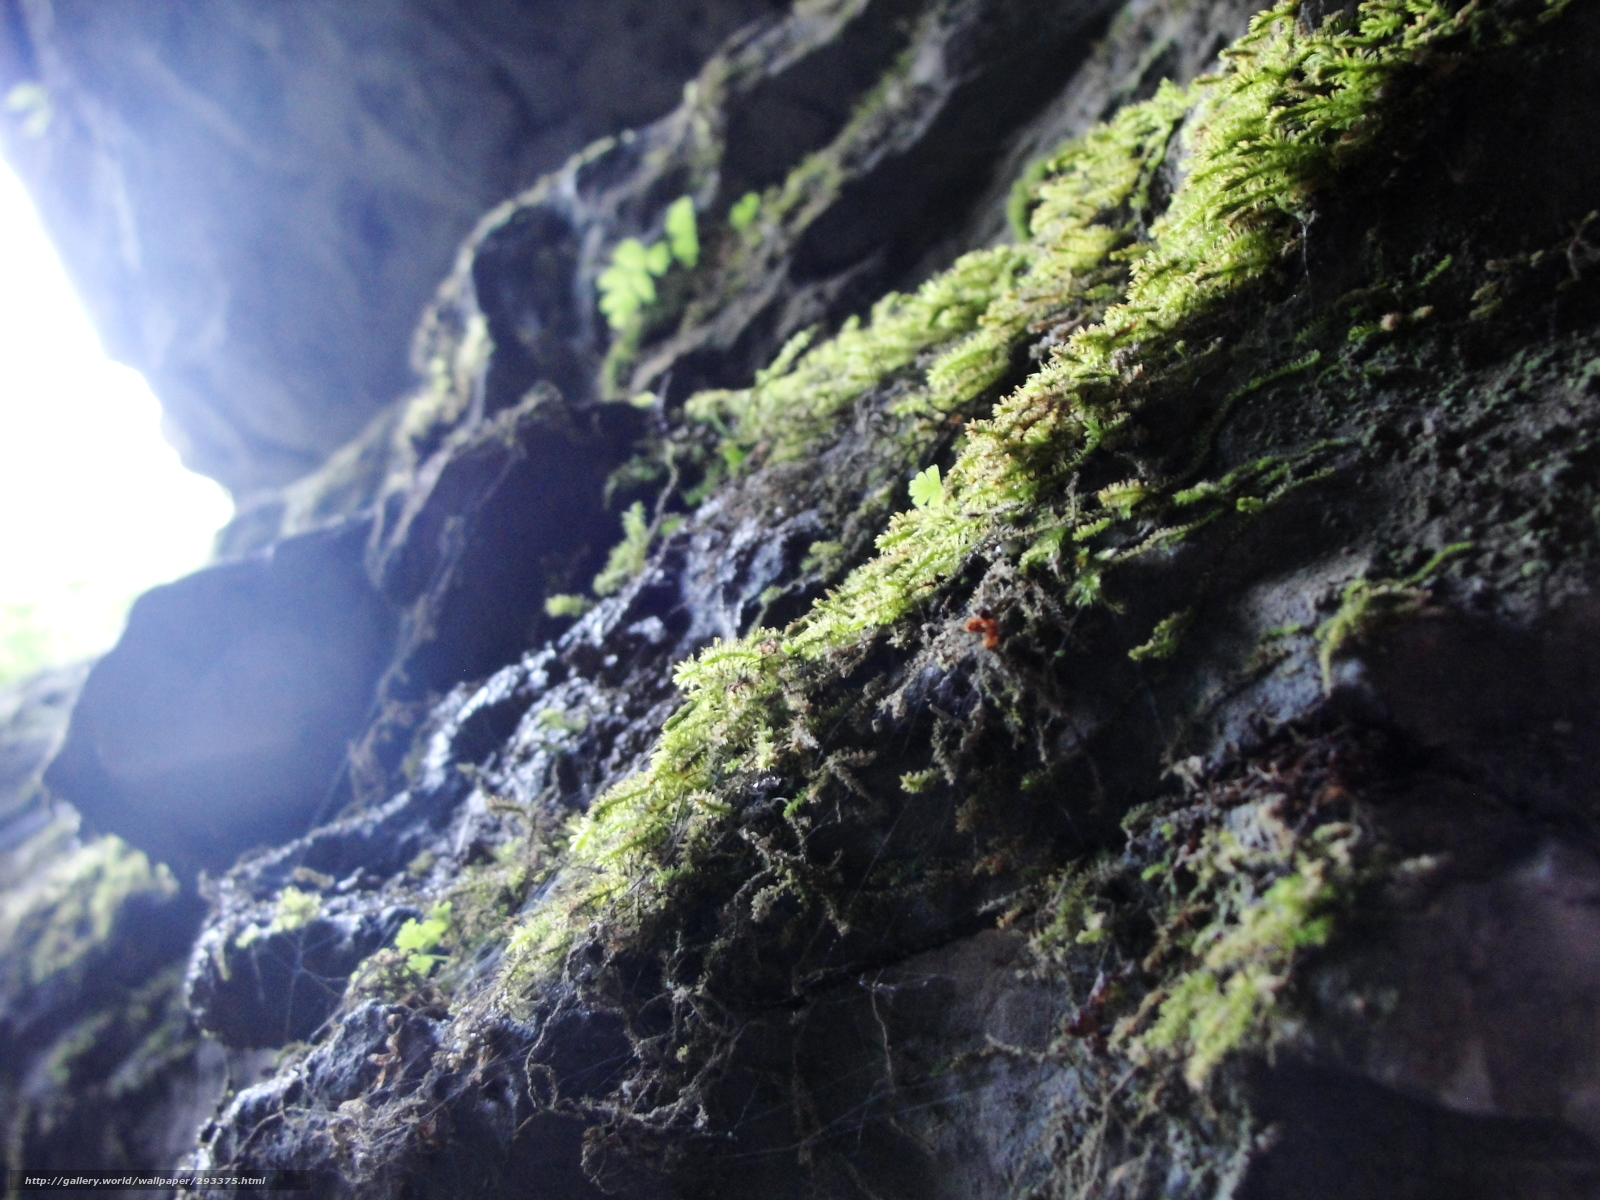
\includegraphics[width=0.99\textwidth]{surface_types/moss.jpg}\\
\caption{Мох}
\label{fig:moss}
\end{subfigure}
\caption{Скользящие поверхности}
\label{fig:slippery_surfaces}
\end{figure}

Представлены габаритные размеры нескольких пещер для определения необходимого запаса хода и размеров компонентов робототехнического комплекса \cite{1960,1963,1969,1971}.

\begin{figure}[H]
\begin{subfigure}{0.8\textwidth}
\centering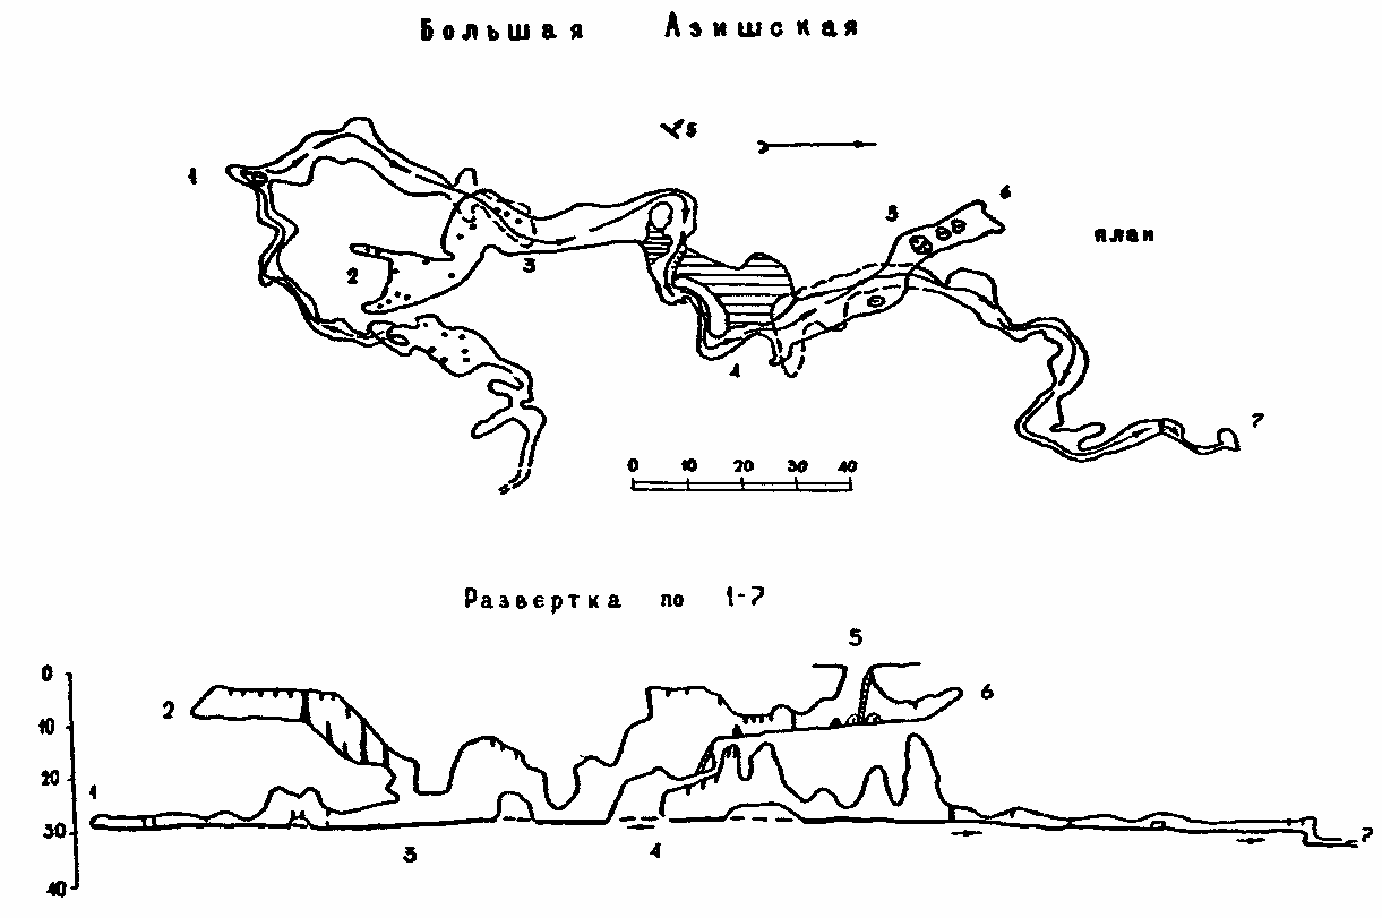
\includegraphics[width=0.7\textwidth]{cave_maps/map1.png}\\
\caption{Большая Азишская пещера}
\label{fig:ice}
\end{subfigure}

\begin{subfigure}{0.8\textwidth}
\centering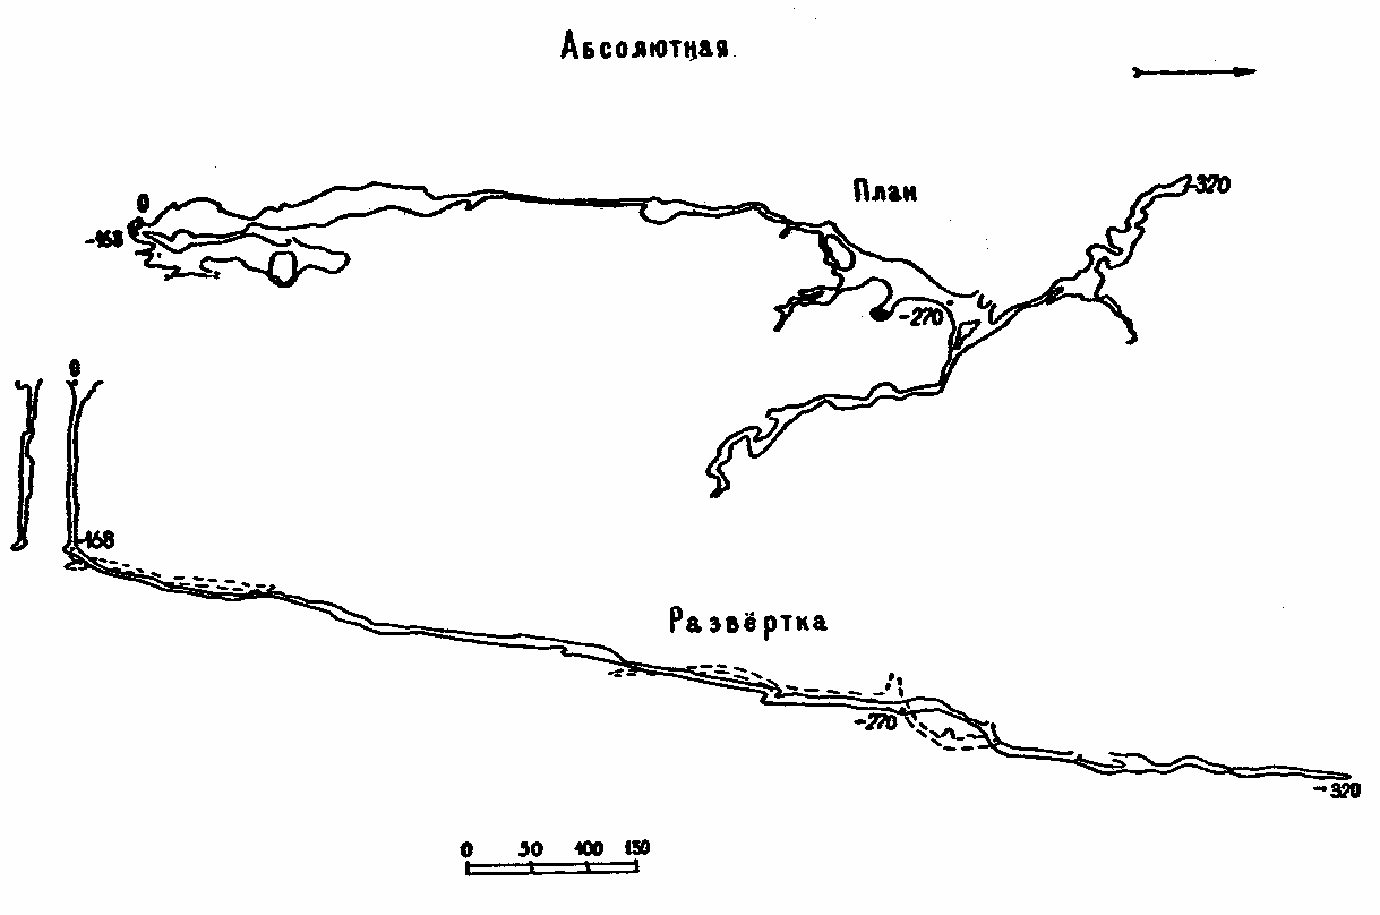
\includegraphics[width=0.7\textwidth]{cave_maps/map2.png}\\
\caption{Абсолютная пещера}
\end{subfigure}

\begin{subfigure}{0.8\textwidth}
\centering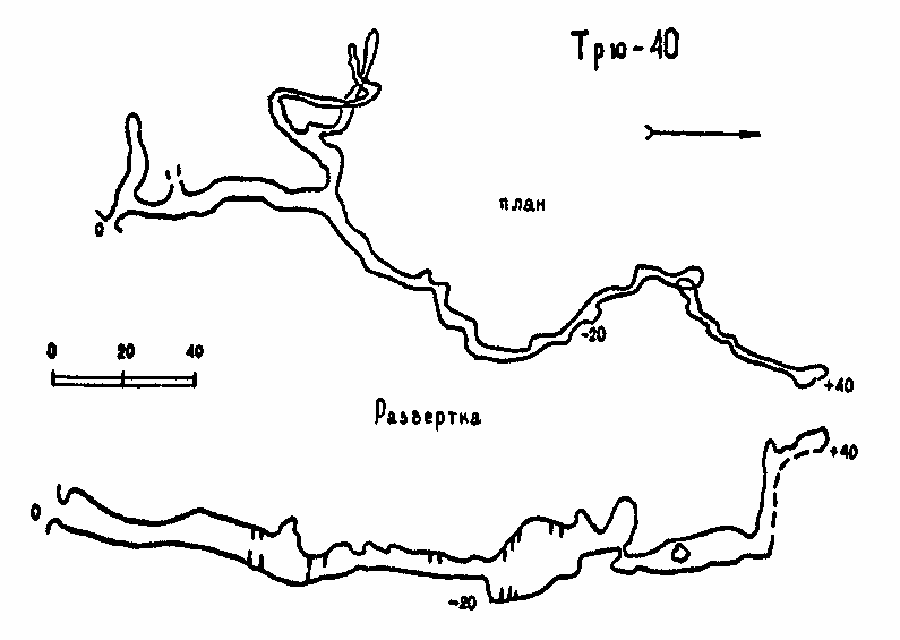
\includegraphics[width=0.7\textwidth]{cave_maps/map3.png}\\
\caption{Трю - 40}
\end{subfigure}
\caption{Примеры карт некоторых пещер}
\end{figure}

Так как существующие карты построены только там, где человек был физически, то таким образом возможно только оценить верхние границы для габаритов робота. Основное преимущество робота это то, что он может пройти в те места, которые недоступны человеку из-за своих размеров.


\section{Классификация сенсорных устройств}
Информация, поступающая с различных сенсорных устройств, используется в системе управления робота для обнаружения и распознавания объектов внешней среды, построения модели окружающих поверхностей, а также для управления движением робота и его манипуляторов при выполнении различных технологических операций. В соответствии с этим, используемые в роботах предложенного класса, группы сенсорных устройств можно описать иначе следующим образом: для выявления свойств внешней среды, отдельных объектов и обеспечения перемещения исполнительных органов \cite{2013,1984,2015}.

К первой из указанных групп относятся сенсорные устройства, предназначенные для выявления различных физико-химических свойств объектов среды, включая, в частности, устройства для выявления параметров рельефа в рабочей зоне мобильных роботов, специальных признаков для обнаружения и распознавания определенных объектов, положения и их ориентации в рабочей зоне относительно робота и т. п.

Ко второй группе относятся датчики обратной связи (положения, скорости, ускорения), усилий, возникающих при взаимодействии робота с внешней средой, прикосновения, проскальзывания и т. д.

Такое разделение сенсорных устройств достаточно условно, поскольку, например, сенсорные устройства первой группы могут быть использованы и для определения положения захвата манипулятора робота в рабочей зоне, т. е. играть роль датчиков обратной связи при управлении движением.

Сенсорные устройства робота могут воспринимать информацию на различных расстояниях от ее источника. По этому признаку сенсорные устройства делятся на сверхближние, ближние, дальние и сверхдальние (работающие вне рабочей зоны).

Сенсорные устройства сверхближнего действия используют для очувствления захватов и других частей манипуляторов, а также корпуса робота. Они позволяют фиксировать их контакт с объектами внешней среды (тактильные датчики), измерять усилия, возникающие в месте взаимодействия (силометрические датчики), фиксировать проскальзывание объектов.

Сенсорные устройства ближнего действия обеспечивают получение необходимой информации в непосредственной близости от робота, но бесконтактным способом. К таким устройствам относятся локационные сенсоры захвата, неконтактные бамперы, различные дальномеры ближнего действия, плотнометры грунта и т. п. Бесконтактные измерительные устройства технически сложнее контактных, но позволяют роботу выполнять задание с большей скоростью, заранее получать информацию о ближайших объектах и соответствующим образом корректировать свои действия.
Сенсорные устройства дальнего действия дают информацию о внешней среде и объеме всей рабочей зоны робота.

Сенсорные устройства сверхдальнего действия применяют главным образом в мобильных роботах. К таким устройствам относятся различные навигационные устройства, координаторы, локаторы и другие оптические, радиотехнические и телевизионные системы.

В бесконтактных сенсорных системах роботов для получения требуемой информации могут быть использованы излучаемые таким устройством специальные сигналы (оптические, радиотехнические, радиационные и т. п.) или естественные излучения среды и отдельных ее объектов. В зависимости от этого различают активные и пассивные сенсорные системы. Первые обязательно включают передающие устройства, излучающие первичный сигнал, и приемные устройства, регистрирующие прямой сигнал, прошедший через среду, или вторичный сигнал, отраженный от объектов среды. Пассивные системы имеют только приемное устройство, а роль излучателя играют сами объекты внешней среды. Поэтому такие устройства технически обычно проще и дешевле, но зато и менее универсальны. Существуют также полуактивные сенсорные устройства, в которых в результате излучения внешней среды инициируется вторичное излучение ее объектов, принимаемое приемными устройствами, как в пассивных системах.
 
Таким образом, на основе классификации были выбраны следующие сенсоры для решения задач перемещения и локализации в пещерах, параллельно определяя тип опорной поверхности. Выбранными семействами сенсоров являются силомоментные, свердальнего действия, бесконтактные, а также датчики обратной связи.

\section{Обзор алгоритмов триангуляций}
Для решения задачи построения карты с помощью тактильного очувствления решено генерировать поверхность на основе полученных точек. Эта задача формулируется следующим образом. Необходимо получить оболочку из набора точек, полученных с лап робота. Одним из примеров оболочки является выпуклая оболочка. Выпуклая оболочка это наименьшее выпуклое множество, содержащее в себе множество $X$. В формализации используется слово оболочка, так как эта поверхность проходима, а оболочка строится на основе облака точек, полученного с пройденной поверхности. 

Для выбора алгоритма необходимо формализовать ограничения и условия, которые присутствуют в конкретной задаче по поостроению карты с помощью тактильного очувствления \cite{ebertInterpolationExtrapolationComparison2014,kumarSurfaceTriangulationSurvey,aurenhammerVoronoiDiagramsSurvey1991}.
\begin{itemize}
    \item Граница вокруг объекта должна быть вогнутой формы, а не выпуклой. Более подробно этот тезис объясняется в главе \nameref{ch:ch4}.
    \item Плотность полученного облака точек не играет роли.
\end{itemize}

Область интерполяции \cite{brooksCharacterizingDomainRegression1988,patelLinearProgramDetect1995,baranyiEffectsParameterizationPerformance1996,haffnerEscapingConvexHull2001,kingDangersExtremeCounterfactuals2006} --- это когда одна группа объектов или набор данных является базой для определения диапазона значений для интерполяции и заключена в некую границу выпуклой формы. Область за пределами этой границы или корпуса обозначается как область экстраполяции. Обычно эту область называют выпуклой оболочкой. В редких случаях авторы применяют определение экстраполяции к области между несколькими группами объектов. Пример использования метода кластеризации для определения новых точек данных в области экстраполяции для обнаружения повреждений при изменяющихся условиях окружающей среды и эксплуатации для мониторинга состояния конструкций.

Существуют множество алгоритмов, которые рассматривают случай, когда у одной группы объектов оболочка не является выпуклой. \cite{rejerHypertubePossibleInterpolation2006,j.a.leonardUsingRadialBasis1992,verleysenLearningHighdimensionalData2001}.

Для решения задачи построения карты необходимо использовать алгоритмы, основанные на получении вогнутой оболочки. Чаще всего такие алгоритмы используют за основу выпуклую оболочку и модифицируют ее.

Первыми алгоритмами для вычисления выпуклых оболочек были Алгоритм Грэхема \cite{grahamEfficientAlgorithDetermining1972} и Алгоритм Джарвиса \cite{jarvisIdentificationConvexHull1973}, которые были усовершенствованы в \cite{chanOptimalOutputsensitiveConvex1996}. Все эти алгоритмы были ограничены проблемами низкой размерности. 

Для получения выпуклой оболочки большей размерности был предложен алгоритм быстрой оболочки \cite{clarksonApplicationsRandomSampling1988}.Более современные алгоритмы применимы к более комплексным областям применения. К примеру такими алгоритмами являются <<динамические выпуклые оболочки>>, <<аппроксимация оболочки для больших наборов данных>>, <<алгоритмы выпуклых оболочек для больших размерностей>> \cite{brodalDynamicPlanarConvex2002,khosravaniSimpleAlgorithmConvex2013,zhongFindingConvexHull2014}. Так как для задач построения карты для беспилотных автомобилей требуется решения в режиме реально времени, авторы разрабатывают усовершенствования производительности алгоритмов путем распараллеливания и использования графического процессора (GPU) для определения внутренних точек \cite{zhongFindingConvexHull2014,cintraSpeculativeParallelizationRandomized2004,cintraSpeculativeParallelizationRandomized2004,tangSMI2012Full2012,tzengFindingConvexHulls2012}.

Для построения вогнутых оболочек существует несколько различных подходов к вычислению границ произвольной формы. Основные концепции алгоритмов построения вогнутых оболочек основаны на методах ближайших соседей, kernel функциях или триангуляции Делоне. Хотя это не совсем алгоритм для построения вогнутой оболочки, существует также подход, который с помощью статистики определяет признаки новизны. В итоге данный подход решает ту же проблему. 

Известным алгоритмом для построения вогнутой оболочки является $\alpha$-shapes \cite{edelsbrunnerShapeSetPoints1983,edelsbrunnerThreedimensionalAlphaShapes1992}. Это обобщение вогнутой оболочки, где $\alpha$ - параметр, и по мере приближения $\alpha$ к 0, $\alpha$-оболочка приближается к обычной выпуклой оболочке. $\alpha$-оболочки строятся из диаграмм Вороного. Есть альтернатива --- $\chi$-фигуры \cite{duckhamEfficientGenerationSimple2008}. Алгоритм $\chi$-форм является простым, гибким и эффективным для построения возможно невыпуклого простого многоугольника, который характеризует форму набора входных точек на плоскости, называемую характерной формой. Вместо диаграмм Вороного алгоритм основан на триангуляции точек по методу Делоне. Есть еще модификации на основанные на алгоритме Грэхема \cite{xuConcaveHullAlgorithm2010} с унаследованными ограничениями. 

Другой подход представлен Парком \cite{parkNewConcaveHull2012}, который начинается с выпуклой оболочки и применяет алгоритм "копания". Благодаря работе \cite{j.a.leonardUsingRadialBasis1992} и  метода машинного обучения  SVM, возник новый класс методов обнаружения. Однако одноклассовые SVM не дают точной оболочки, и для различения между внутренним и внешним необходимо задать порог. С дополнительной информацией возможна двухклассовая SVM. 

Для вычисления независимых оболочек для нескольких групп объектов предлагается алгоритм с использованием алгоритма кластеризации общих ближайших соседей (SNN) , который вычисляет оболочку для каждой группы, применяя подход k-nearest neighbors (kNN) \cite{moreiraConcaveHullKnearest2007,ertozNewSharedNearest2002,chauBorderSamplesDetection2011,xiaBORDEREfficientComputation2006}.

\section{Обзор разработанной системы}
\begin{figure}[H]
    \centering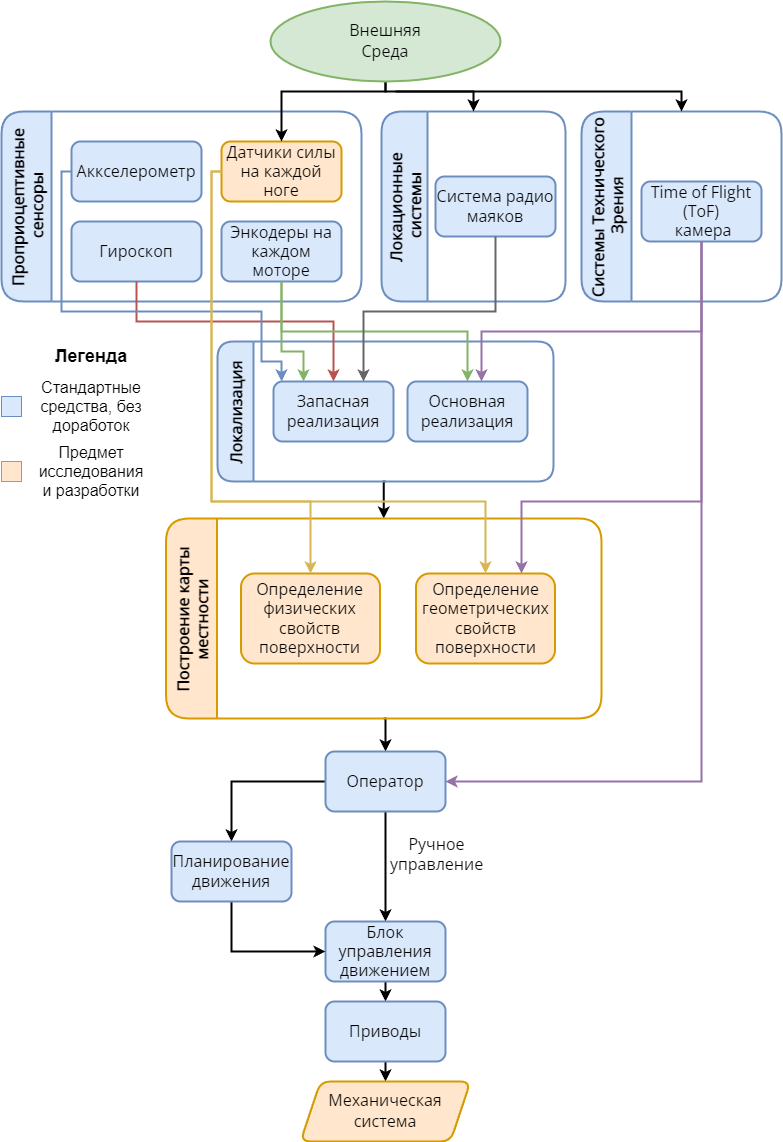
\includegraphics[height=22cm,width=1\textwidth,keepaspectratio]{main_diag.drawio.png}
    \caption{Структурная схема разрабатываемой системы}
    \label{fig:diag_system.png}
\end{figure}

Оранжевым цветом выделены те элементы, которые были разработаны и изучены, остальные --- взяты готовые решения. Жирными стрелками показаны те блоки, на которых сделан упор в диссертации.

Верхний блок это внешняя среда, то есть вся информация о внешнем мире, с которой работает робот. Следующая группа блоков связана с сенсорами. Часть из них --- проприцептивные, то есть внутренние датчики, такие как гироскоп, аккселерометр, энкодеры и датчики силы. Разработке последнего элемента посвящена целая глава \nameref{ch:ch3}. Так же есть система технического зрения, в представленном роботе это камеры Time of Flight (ToF). Это камера, которая может выдавать облако точек. А так же глобальная навигация с помощью радио маяков, которые робот выбрасывает во время своего перемещения, таким образом строя систему из маяков. Данная задача вынесена за рамки работы.

Следующим слоем является локализация. Она основана на данных, полученных с сенсоров. В данной системе 2 локализации, основная, более точная. Основанная на камере, и запасная --- основанная на IMU, датчиках силы и системе маяков. Это та система, в которой наиболее выигрышно смотрится предложенное решение.

Следующий блок, который реализован и разработан автором --- построение модели местности. Он состоит из трех блоков, которые описаны в соответствующей главе \nameref{ch:ch4}.

Полученные данные попадают оператору, и оператор может управлять роботом, как в ручном режиме, так и просто задав точку, куда роботу нужно прийти. Эта высокоуровневая команда идет в блок управления движением, а дальше это уже реализуется с помощью механической системой.

В работе научная новизна представлена в блоках, связанных с очувствлением: датчики силы, построение карты местности, определение физических свойств объекта. Для улучшения текущих решений необходимо разбираться в самых современных алгоритмах и концептах, связанные с этой тематикой.

\section{Применимость системы}
Необходимо понимать возможности робототехнической системы. Следующая задачей является формализация условий ее применимости. Из полученных условий возможно определить конкретные существующие места, где такую систему возможно применить.

Как итог, был сделан вывод, что данная система может использоваться в узких пещерах, где не может пролезть человек. Шагающие машины обладают лучшей проходимостью, чем гусеничный или колесный тип движителя, поэтому его использования в местах, где есть большой перепад высот и нет возможности набирать высокую скорость из-за обилия препятствий обоснован. Датчики силы на основе Velostat являются самыми подходящими для разрабатываемой робототехнической системы по причине соотношения цены и точности. Для получения геометрической поверхности модифицируется алгоритм создания вогнутой оболочки с помощью триангуляции Делоне и alpha геометрии. Физические свойства поверхности определяются с помощью обучения стендовой установки на различных типах поверхности с использованием алгоритма SVM и kNN.